\chapter{Project Management}
The following chapter goes into detail about the project management and the decisions that were made. This includes decisions regarding what development methods to use, responsibilities, communication, planning and risk analysis.

\section{Development method}
It is important to chose a development method that fits the project based on the customer, the development team and the project to be developed.

\subsection{Considerations}
In approaching the subject, the team wanted a development method that could adapt to changes in the requirements, as it was not clear whether Vitensenteret would change them or not. It was decided that the team would meet the customers every other week.

\subsection{Reasoning}
Based on the prestudy, described in chapter 2, in addition to the considerations described above, the team made some decisions about the development method. It became clear early that scrum was a wise choice. The group  

Scrum was also a development method which all members of the group had previous experience with.\\
\\
With the agile properties and the iterative work process scrum has, it fit very good into the project. The group needed to have a good dialog with the customer, since the requirements were not clearly defined in advance. The close communication with was essential in order to make an application that satisfied their wishes. Pair programming was also widely used. This was done in order to share knowledge and to hopefully achieve the advantages of Pair Programming listed in chapter2.3.4 

\subsubsection{Adaptions}
In order for scrum to work as good as possible for the group, a few adaptions were made. Since the meetings with the customer were every other week, the duration of a sprint was set to two weeks. The sprint ended right before the customer meeting, and a new one started the day after. This was done in order to be able to present new functionality to the customer at every meeting. Since all the team member took two other courses in parallel to this project, it was decided to have daily scrum meetings four times a week, instead of every day. Instead of having daily stand-up meetings an activity plan was made using cards on Trello. The activity plan kept track what tasks here, when they were done and by whom they were done. The activity plan also replaced the standard scrum board one often finds in scrum projects 

\section{Team organization}
It is important to have a structured and well organized team. This section contains information about the different aspects of team organization, and how the group organized themselves.

\subsection{Agreement of Cooperation}
All the team members agreed on the fact that good grade was something to aim at. The goal was grade A. In order to easier achieve that, a contract was made. The contract set the terms for how the group was going to work; when the group meetings should be, what was considered valid absence, how many hours each member was expected to spend on the project, and etc. The contract was made in order to minimize the extent of conflicts, disagreements and misunderstandings. The contract was written early in the period and signed by everyone right after.

\subsection{Team roles}
Traditionally a team consists of members with specific and clear roles. These include, but are not limited to group leader, architect, designer, developer and tester. Seeing as this is a student project, the members roles are not as clear because all members want to gain an understanding for the different aspects of the project and acquire the necessary skills and knowledge to be able to participate in any given role in the future. However, areas of responsibility have been distributed to the team members that are best equipped within the different areas of expertise.

\subsubsection{Role description}
It was important to divide the different roles between the group members, so that everyone always knew who to contact about what.\\
\\
\textbf{Group leader:} The group leader had responsibility for contact with the customer and the supervisor. Also to ensure project progress and to meet deadlines. The group leader was the chairman of the group meetings.\\
\\
\textbf{System architect:} \TODO{Vet ikke hva jeg skal skrive her.}\\
\\
\textbf{Designer:} The designer was responsible for making a consistent graphical layout for the application, and to make the application intuitive to use.\\
\\
\textbf{Tester:} The tester had responsibilities regarding the testing done in the project. This includes writing tests, making sure the other group members wrote tests, and conducting user tests and the acceptance test with the customer.\\
\\
\textbf{Backend developer:} Main responsibility was to develop the backend for the project. Although this was a rather small task, it was important to have a responsible for it.\\
\\
\textbf{Frontend developer:} The frontend developer was responsible for the development of the frontend. In other words, responsible for making the idea and design into code.

\subsubsection{Role distribution}
This was how the roles were distributed in the proejct.\\
\\
\textbf{Group leader:} Didrik Pemmer Aalen\\
\\
\textbf{Architect:} Bjor Løyning Byrkjedal \\
\\
\textbf{Designer:} David André Årthun Bakke\\
\\
\textbf{Test leader:} Kristian Svoren\\
\\
\textbf{Backend developer:} Nicolas Almagro Tonne\\
\\
\textbf{Frontend developer:} Oscar Conrad

\subsection{Communication}
It was important to choose communication tools that worked for all members of the group. \\
\\
The group decided to use Facebook as the main source of communication inside the group. In the beginning both Facebook groups and Facebook chat was utilized by the group, but as time went by, the usage of the Facebook group declined. This was because of the simplicity of using the Facebook chat.\\
\\
The main channel for communication with both the customer and the supervisor was email. This was also used for some of the communication in the group, e.g. when information from the supervisor or the customer had to be spread to the rest of the group, it was often sent via email.\\
\\
In addition to communicating with the customer per email, there were biweekly meetings with them. When communicating with Vitensenteret, the group was in contact with five different people. The director, Arnfinn Stendal Rokne, the IT manager Markus Nygård, the educator, Rannvei Sæther, the designer, Svein Erling Lode and Martin Kulhawczuk, head of communication.


\section{Project planning}
Planning a project consists of, among other, dividing bigger tasks into smaller tasks, have an overview over all the tasks in the project, estimate the time of the project as a whole, and estimating how much time every small task will take.

\subsection{Work breakdown structure}
A work breakdown structure is hierarchical decomposition of the work to be done in a project. It is composed of two elements: the WBS tree and a table which defines the chunks of work to be done \cite{wbs}\cite{wbs2}.\\
\\
In the beginning of the project, after deciding what idea to use, the group tried to break the project into packages. This resulted in the work breakdown structure tree in Figure 3.1. Each chunk in the work breakdown structure tree is described in detail in Table 3.1.\\
\\
\begin{figure}[H]
    \includegraphics[width=\textwidth]{images/WBS.png}
    \caption{Work Breakdown Structure tree}
\end{figure}

\begin{center}
\begin{table}[H]
\caption{Work breakdown structure}
\begin{tabular}{| m{2cm} | m{5cm} | m{5cm} |}
\hline
\textbf {WBS code} & \textbf {Name} & \textbf{Definition} \\
\hline
     & Vitensenteret - Application & All the work done in order to create the application that Vitensenteret wanted for both iOS and Android.   \\
    \hline
    1 & Project management & All the work done with planning and managing the project. \\ 
    \hline
    1.1 & Customer meetings & Meetings with the customer to show project status and discuss ideas, requirements and changes. \\
    \hline
    1.2 & Group meetings & Group meetings have discussions about the project, distribute work and work together with the project.\\
    \hline
    1.3 & Status reports & Writing status reports. \\
    \hline
    1.4 & Risk planning & Defining the risk for the project and analysing them. \\
    \hline
    1.5 & Time estimation & Estimate the time needed to complete the different tasks. \\
    \hline
    1.6 & Team roles & Distribute roles to the team members. \\
    \hline
    2 & Prestudy & The work done in order to gather information about the project. \\
    \hline
    2.1 & Idea researching & The work done with coming up with ideas for the application. \\
    \hline
    2.2 & Development research (Tools, frameworks, etc) & The work done to find the right tools and framework to develop the application with. \\
    \hline
    2.3 & Requirement specification & Defining the requirements for the application and making use cases for the different requirements. \\
    \hline
    3 & Design & The total workload for designing the application. \\
    \hline
\end{tabular}\\
Continues on the next page.
\end{table}
\end{center}
\begin{center}
\begin{table}[H]
Continued from the previous page.\\
\begin{tabular}{| m{2cm} | m{5cm} | m{5cm} |}
\hline
\textbf {WBS code} & \textbf {Name} & \textbf{Definition} \\
    \hline
    3.1 & Sketching the design on paper / computer & The initial design process. Make the design for the application before implementing it. \\
    \hline
    3.2 & Implement the design & Code the design for the application. \\
    \hline
    4 & Development & Coding the functionality for the application, as well as writing documentation. \\
    \hline
    4.1 & Implement functionality to the design & Create logic for the implemented design, so that the application works. \\
    \hline
    4.2 & Implement beacon functionality & Make the application work with beacons. \\
    \hline
    4.3 & Implement database / backend functionality & Create the database the holds the robots in the application. \\
    \hline
    4.4 & Write Documentation & Write installation guide and user manual. \\
    \hline
    5 & Testing & All the work put into testing the application. \\
    \hline
    5.1 & Unit testing & Testing every part of the application separately. \\
    \hline
    5.2 & User testing & Let people in the targeted group test the application and come with feedback.\\
    \hline
    5.3 & System testing & Test the system when all units are combined. \\
    \hline
    5.4 & Acceptance testing with Vitensenteret & Let Vitensenteret try the application and come with feedback.\\
    \hline
    6 & Project closure & The work put into completing the project. \\
    \hline
    6.1 & Project report & Finish the final report. \\
    \hline
    6.2 & Product delivery & Deliver the product to the customer and the course staff. \\
    \hline
    6.3 & Publish application in Google Play and Apple Appstore & Publish the application so that it can be used. \\
    \hline
\end{tabular}
\end{table}
\end{center}

\subsection{Time estimation}
An important aspect of project planning was time estimation. This included everything from estimating the project as a whole to estimating the smaller tasks in the project. The group started out with making a GANTT-diagram based on the work breakdown structure. 
\subsubsection{GANTT}
The group tried to estimate how much time each of the packages would take in the project. This resulted in the GANTT-diagram in Figure 4.2. See Appendix \TODO{x} for a full-sized GANTT diagram.\\
\\
\begin{figure}[H]
    \centering
    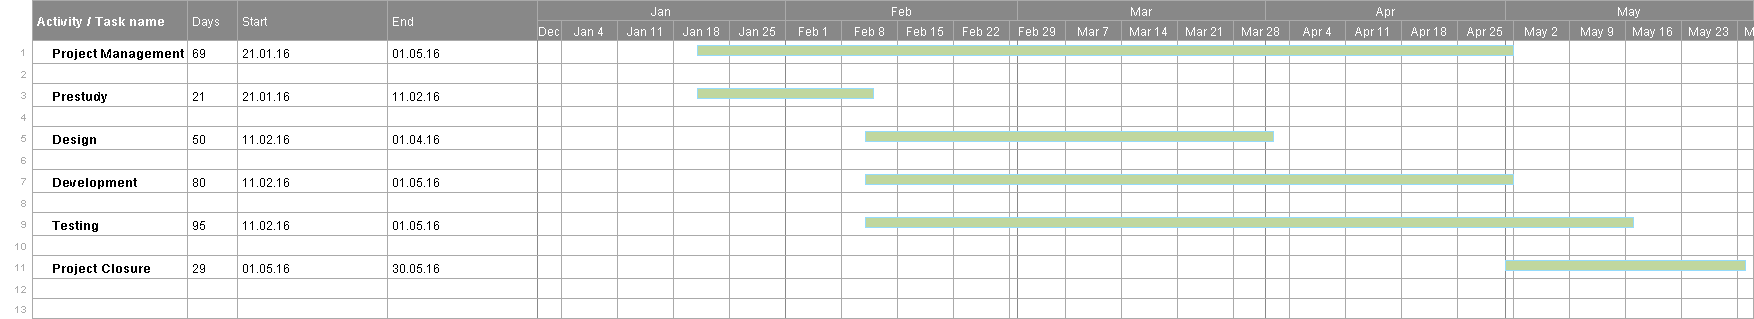
\includegraphics[width=\textwidth]{images/gantt1.png}
    \caption{GANTT diagram.}
\end{figure}

\subsubsection{Task estimation}
After estimating the project as a whole, the group tried to break the design and development process into smaller and more manageable tasks. The group decided to use planning poker to estimate the smaller tasks. Planning poker was a consensus based, gamified technique for estimating workload in terms of hours. The initial estimations made with planning poker can be seen in Table 3.2. In this estimation the group tried to find all the tasks linked to design and development in the project, but there was some additions and deletions of tasks later in the process.\\
\\
The first activity plan the group made was based on the estimations made with planning poker, but this was the only activity plan made based on these estimations. After finishing the first activity plan, the group discovered that the initial estimations done with  planning poker were not accurate. The group decided that planning poker did not work for the group and conducted therefore the time estimated in a different manner after the first activity plan was finished. \\
\\
After the first activity plan was finished, the group was more experienced with the tools and frameworks, thus making the group more fit to make estimations based on experience. See Appendix \TODO{X} for an example of an activity plan used in the project.

\begin{center}
\begin{table}[]
\caption{Initial estimation made with planning poker}
\begin{tabular}{ |l|r| } 
\hline
\textbf {task} & \textbf {Estimation in hours} \\
\hline


Learn technologies (Self study) (Cordova) &
32 \\
\hline
Design general layout &
18 \\
\hline
implement functionality for the general layout &
20 \\
\hline
Design color-minigame layout &
24 \\
\hline
implement functionality for color-minigame &
5 \\
\hline
Design layout for quiz-minigame &
10 \\
\hline
implement functionality for quiz-minigame &
40 \\
\hline
Design layout for shortest path-minigame &
10 \\
\hline
implement functionality for shortest path-minigame &
16 \\
\hline
Design layout for table of elements-minigame &
10 \\
\hline
implement functionality for table of elements-minigames &
7 \\
\hline
Design layout for water-minigame &
24 \\
\hline
implement funtionality for water-minigame &
23 \\
\hline
Design layout for memory-minigame &
16 \\
\hline
implement functionality for memory-minigame &
18 \\
\hline
Design layout for sound-minigame &
25 \\
\hline
implement functionality for sound-minigame &
22 \\
\hline
Design different robot-parts &
? \\
\hline
Setting up database &
22 \\
\hline
Handle data from database in application &
25 \\
\hline
Learn beacon-technology &
? \\
\hline
Make the application communicate with beacons &
? \\
\hline
Make superclasses with possibilities for inheritance &
35 \\
\hline
Testing &
110 \\
\hline
Total &
512 \\
\hline


\hline
\end{tabular}
\end{table}
\end{center}


\section{Risk analysis}
Table 4.3 shows the risks identified by the group, and the likelihood, impact and importance of the specified risks to happen. Likelihood reflects how likely the group thought the risk would be during the project period. Impact reflects how high the group considers the consequences of the risk. Importance is found by multiplying likelihood and impact. The higher number importance get, the more important is it to avoid the risk.

\begin{center}
\begin{table}[h]
\caption{Risk analysis}
\begin{tabular}{ | m{2.2cm} | m{1cm} | m{1.2cm} | m{1.2cm} | m{2cm} | m{2.2cm} | }
\hline
\textbf{Description} & \textbf{Likeli- hood} & \textbf{Impact} & \textbf{Impor- tance} & \textbf{Preventive action} & \textbf{Remedial action}\\
\hline
    Misestimation of work/time & 7 & 5 & 35 & Read about time estimation & Continuous re-estimation of workload and open dialogue with the customer. Keep the possibility to simplify the project\\
\hline
    Loss of work or data & 7 & 5 & 35 & Save and do backups. Use github often. & Try to recover lost data and/or work. \\ 
\hline
    Serious illness & 3 & 8 & 24 & Be safe & Speak to customer and try to simplify the project, as well as redistribute work task between remaining members\\
    \hline
    \end{tabular}\\
    Continues on the next page.
\end{table}
\end{center}

\begin{center}
\begin{table}[h]
Continued from the previous page.\\
\begin{tabular}{ | m{2.2cm} | m{1cm} | m{1.2cm} | m{1.2cm} | m{2cm} | m{2.2cm} | }
\hline
\textbf{Description} & \textbf{Likeli- hood} & \textbf{Impact} & \textbf{Impor- tance} & \textbf{Preventive action} & \textbf{Remedial action}\\
\hline
    Problems with working with new technology & 6 & 4 & 24 & Read documentation and prepare well. & Trial and error, discarding the technology. Use technology the group is familiar with.\\
\hline
    Team members not contributing & 3 & 8 & 24 & Agree on a contract that the group members all had to sign. & contact regarding team member and the course leader.\\
\hline
    Change in project requirements & 3 & 7 & 21 & Open dialogue with the customer and to make a good plan. & Adapt to changes\\
\hline
    Problems with the customer & 1 & 8 & 8 & Keep contact with the customer. & Contact our supervisor and try to contact the customer.\\
\hline
\end{tabular}
\end{table}
\end{center}
\subsection{Changes}
As time goes by in a project, it is possible to see that other risks were at hand, and change the risk analysis accordingly. The changes that had to be done for this project involves team members being ill over time and thus not able to contribute to the project, team members going away for a while, making team meetings and some communication hard to perform. See Table \ref{addedrisk} for the added risks to the analysis.\\
\\
\begin{center}
\begin{table}[H]
\caption{Added risks to the risk analysis}
\begin{tabular}{ | m{2.2cm} | m{1cm} | m{1.2cm} | m{1.2cm} | m{2cm} | m{2.2cm} | }
\hline
\label{addedrisk}
\textbf{Description} & \textbf{Likeli- hood} & \textbf{Impact} & \textbf{Impor- tance} & \textbf{Preventive action} & \textbf{Remedial action}\\
\hline
    Less serious illness & 9 & 6 & 54 & Try to stay healthy and avoid contageous scenarios. & Work from home. Focus on good communication. Help each other with the workload.\\
\hline
    Change in the requirements & 6 & 7 & 42 & Have an active conversion with the customer. & Try to adapt to adapt to the changes. If time makes it impossible to implement the changes, tell the customer that it is not possible.\\
\hline
\end{tabular}
\end{table}
\end{center}

